\documentclass[11pt]{article}

% --------------------
% Packages
% --------------------
\usepackage[margin=1in]{geometry}
\usepackage{amsmath, amssymb, amsthm, mathtools}
\usepackage{bm}
\usepackage{graphicx}
\usepackage{booktabs}
\usepackage{enumitem}
\usepackage{microtype}
\usepackage{xcolor}
\usepackage{hyperref}
\usepackage[numbers,sort&compress]{natbib}

% --------------------
% Formatting
% --------------------
\hypersetup{
    colorlinks=true,
    linkcolor=blue,
    citecolor=blue,
    urlcolor=blue
}

\setlength{\parindent}{0pt}
\setlength{\parskip}{0.75em}

% --------------------
% Theorem environments
% --------------------
\newtheorem{proposition}{Proposition}
\newtheorem{remark}{Remark}
\newtheorem{definition}{Definition}

% --------------------
% Macros
% --------------------
\newcommand{\R}{\mathbb{R}}
\newcommand{\one}{\mathbf{1}}
\newcommand{\LN}{\operatorname{LN}}
\newcommand{\DyT}{\operatorname{DyT}}
\newcommand{\rank}{\operatorname{rank}}
\newcommand{\diag}{\operatorname{diag}}
\newcommand{\sech}{\operatorname{sech}}
\newcommand{\tr}{\operatorname{tr}}
\newcommand{\softmax}{\operatorname{softmax}}
\newcommand{\srank}{\operatorname{srank}}
\newcommand{\kappaeff}{\kappa_{\varepsilon}}

% --------------------
% Title
% --------------------
\title{\vspace{-1em}
Are Normalization-Free Transformers Numerically Similar?
}

\author{Kyle Luo\\
Massachusetts Institute of Technology}

\date{}

\begin{document}

\maketitle

\begin{abstract}
Recent work on Dynamic Tanh (DyT) shows that transformer normalization layers can often be replaced by the elementwise map \(\DyT(x)=\tanh(\alpha x)\) while preserving strong task performance. This paper asks whether that replacement also preserves the numerical structure of the matrices inside a transformer. We compare core, non-affine LayerNorm and DyT maps via the effective condition number, stable rank, and rank-$k$ approximation error of feature matrices, Gram matrices, and attention score matrices from DistilBERT, together with a first-order perturbation bound on the attention scores. Theoretically, LayerNorm is a projection-rescaling map: it removes the all-ones direction, fixes row norms, and forces $G_{ii}=d$. DyT is a coordinatewise saturation: it bounds rows in $[-1,1]^d$ and contracts saturated coordinates without removing global shift or scale. Empirically, the sharpest distinction is the Gram diagonal: LayerNorm fixes it at $d$ up to the $\varepsilon$ regularization, while DyT produces input-dependent diagonals controlled by $\alpha$. Rank-$32$ approximation error and the relative attention perturbation $\|\Delta S\|_F/\|S\|_F$ are close across transforms; stable rank shows a consistent gap (DyT $>$ LN at every layer); the effective condition number separates the maps but with no consistent layer ordering. Thus task-level similarity between LayerNorm and DyT does not imply full numerical equivalence.
\end{abstract}

\section{Introduction}

Transformers have become a central architecture in modern machine learning, with applications across language modeling, computer vision, and sequence modeling. A standard component of transformer architectures is LayerNorm, which is typically treated as a default part of the transformer block rather than as a separate numerical operation to be analyzed. For a feature vector \(x\in\mathbb{R}^d\), LayerNorm computes
\begin{equation}
    \mu(x)=\frac{1}{d}\sum_{j=1}^d x_j,
    \qquad
    \sigma(x)^2=\frac{1}{d}\sum_{j=1}^d (x_j-\mu(x))^2
\label{eq:ln-statistics}
\end{equation}
and maps
\begin{equation}
    \LN(x)=\frac{x-\mu(x)\mathbf{1}}{\sigma(x)}
\label{eq:layernorm}
\end{equation}
Thus, LayerNorm is a nonlinear rowwise transformation applied repeatedly to hidden-state matrices inside the model.

Recent work has increasingly questioned which parts of normalization are actually necessary in transformers. The original Transformer used normalization together with residual connections and scaled dot-product attention \cite{vaswani2017attention}, and LayerNorm was introduced as a normalization method based on per-example, within-layer statistics rather than batch statistics \cite{ba2016layer}. RMSNorm weakens LayerNorm by removing the recentering operation while keeping a rescaling mechanism, suggesting that mean subtraction is not always essential for strong performance \cite{zhang2019rmsnorm}. Other work studies normalization through placement and scaling: analyses of Pre-LN and Post-LN transformers show that LayerNorm placement affects gradient behavior and training stability, while NormFormer and DeepNet modify normalization or residual scaling to improve optimization and enable deeper models \cite{xiong2020layernorm,shleifer2021normformer,wang2022deepnet}. Dynamic Tanh (DyT) pushes this line of work further by replacing normalization layers with the coordinatewise map
\begin{equation}
    \DyT(x)=\tanh(\alpha x),
    \qquad
    \tanh(t)=\frac{e^t-e^{-t}}{e^t+e^{-t}}
\label{eq:dyt}
\end{equation}
where \(\alpha>0\) is a scalar parameter \cite{zhu2025transformers}. In this sense, DyT is not just another normalization variant: it replaces a rowwise normalization map with an elementwise saturating nonlinearity.

These works provide strong evidence that normalization is not a settled primitive in transformer design. However, they mostly evaluate normalization through machine learning quantities such as accuracy, loss, convergence, gradient behavior, or benchmark performance. They do not directly address whether different normalization choices induce the same matrix-level structure inside the model. To study this question, we consider the matrices naturally associated with a transformer layer. We write \(X_\ell\in\mathbb R^{n\times d}\) for the feature matrix at layer \(\ell\), whose rows are token or patch representations. Its row Gram matrix is
\begin{equation}
    G_\ell=X_\ell X_\ell^\top,
    \qquad
    (G_\ell)_{ij}=x_i^\top x_j,
\label{eq:intro-gram}
\end{equation}
which records pairwise inner products between representations. Attention uses a second matrix construction. Let
\begin{equation}
    Q_\ell=X_\ell W_{Q,\ell},
    \qquad
    K_\ell=X_\ell W_{K,\ell},
\label{eq:intro-qk}
\end{equation}
where \(W_{Q,\ell}\) and \(W_{K,\ell}\) are the query and key projection matrices at layer \(\ell\). The pre-softmax attention score matrix is
\begin{equation}
    S_\ell=\frac{Q_\ell K_\ell^\top}{\sqrt{d_k}},
\label{eq:intro-attention-score}
\end{equation}
where \(d_k\) is the key dimension. Thus \(G_\ell\) measures geometry directly in feature space, while \(S_\ell\) measures geometry after learned query and key projections.

This paper treats LayerNorm and DyT as numerical maps and asks which matrix-level properties they preserve. LayerNorm behaves as a rowwise projection-rescaling map: its local linearization removes shift and radial perturbation directions. DyT behaves as a coordinatewise saturation map: its Jacobian is diagonal and contracts saturated coordinates. We connect these structural differences to the effective condition number, stable rank, and rank-$k$ approximation error of \(X_\ell\), \(G_\ell\), and \(S_\ell\), and to a first-order perturbation bound on the attention scores, then test them in one controlled DistilBERT case study. The goal is not to rank the two operations universally, but to separate task-level replacement from matrix-level equivalence.

\section{LayerNorm and DyT as Matrix Maps}
\label{sec:maps}

We compare LayerNorm and DyT as maps on feature vectors and feature matrices. Full LayerNorm is usually implemented as
\[
    \LN_{\varepsilon,\gamma,\beta}(x)
    =
    \gamma\odot
    \frac{x-\mu(x)\one}{\sqrt{\sigma(x)^2+\varepsilon}}
    +
    \beta,
\]
where \(\varepsilon>0\) prevents division by zero and \(\gamma,\beta\in\mathbb R^d\) are learned affine parameters. Full DyT similarly has the form
\[
    \DyT_{\alpha,\gamma,\beta}(x)
    =
    \gamma\odot \tanh(\alpha x)+\beta.
\]
In this section, we analyze the core non-affine maps
\[
    x\mapsto \frac{x-\mu(x)\one}{\sigma(x)},
    \qquad
    x\mapsto \tanh(\alpha x).
\]
This matches the controlled comparison used later: we isolate what centering, rescaling, and saturation do to the same feature matrix before learned affine parameters are allowed to change the geometry.

Table~\ref{tab:ln-dyt-map-summary} summarizes the three comparisons developed below. First, LayerNorm imposes exact output constraints, while DyT only bounds coordinates. Second, their Jacobians have different perturbation mechanisms: LayerNorm removes structured directions, while DyT contracts coordinates independently. Third, these row-level differences appear in Gram matrices: LayerNorm fixes the diagonal and trace, while DyT only bounds them.

\begin{table}[h]
\centering
\begin{tabular}{lll}
\toprule
Property & LayerNorm core map & DyT core map \\
\midrule
Operation & Center and rescale row & Apply \(\tanh\) coordinatewise \\
Output constraint & Mean-zero, fixed row norm & Bounded coordinates \\
Row norm & \(\|z\|_2=\sqrt d\) & \(\|y\|_2\leq \sqrt d\) \\
Jacobian structure & Data-dependent, non-diagonal & Diagonal \\
Perturbation effect & Removes shift/radial directions & Contracts saturated coordinates \\
Gram diagonal & \(G_{ii}=d\) & \(0\leq G_{ii}\leq d\) \\
\end{tabular}
\caption{Core matrix-level differences between the non-affine LayerNorm and DyT maps.}
\label{tab:ln-dyt-map-summary}
\end{table}

\subsection{Output Constraints}

LayerNorm is rowwise and data-dependent: the output of each coordinate depends on all coordinates through \(\mu(x)\) and \(\sigma(x)\). The idealized map is only defined when
   $ \sigma(x)>0$
equivalently when \(x\) is not a constant vector. Under this condition, LayerNorm imposes exact geometric constraints.

\begin{proposition}[LayerNorm centers each row]
Let \(x\in\R^d\) satisfy \(\sigma(x)>0\), and let
\[
    z=\LN(x)=\frac{x-\mu(x)\one}{\sigma(x)}
\]
Then
\[
    z^\top \one=0
\]
\end{proposition}

\begin{proof}
This follows immediately from
\[
    z^\top\one
    =
    \frac{\sum_{j=1}^d x_j-d\mu}{\sigma}
    =0,
\]
because \(\mu=d^{-1}\sum_{j=1}^d x_j\).
\end{proof}

\begin{proposition}[LayerNorm fixes row norms]
Let \(x\in\R^d\) satisfy \(\sigma(x)>0\), and let
\[
    z=\LN(x)=\frac{x-\mu(x)\one}{\sigma(x)}
\]
Then
\[
    \|z\|_2^2=d
\]
\end{proposition}

\begin{proof}
By the definition of \(\sigma^2\),
\[
    \|z\|_2^2
    =
    \frac{\sum_{j=1}^d (x_j-\mu)^2}{\sigma^2}
    =
    \frac{d\sigma^2}{\sigma^2}
    =
    d.
\]
\end{proof}
Together, these propositions show that, whenever \(\sigma(x)>0\), LayerNorm maps \(x\) to the sphere of radius \(\sqrt d\) inside the mean-zero subspace. Equivalently, if \(X_{\LN}\in\mathbb R^{n\times d}\) is obtained by applying LayerNorm rowwise, then
\begin{equation}
    X_{\LN}\one_d=\mathbf 0_n
\label{eq:ln-mean-zero-matrix}
\end{equation}
where \(\one_d\in\mathbb R^d\) is the all-ones vector and \(\mathbf 0_n\in\mathbb R^n\) is the zero vector. Thus every normalized token representation lies in the mean-zero subspace of \(\mathbb R^d\), and every row has Euclidean norm \(\sqrt d\).

LayerNorm also has exact invariances. For any \(a\in\R\),
\begin{equation}
    \LN(x+a\one)=\LN(x),
\label{eq:ln-shift-invariance}
\end{equation}
and for any \(b>0\),
\begin{equation}
    \LN(bx)=\LN(x).
\label{eq:ln-scale-invariance}
\end{equation}
For \(b<0\), \(\LN(bx)=-\LN(x)\). Thus LayerNorm discards global shift and positive radial scale, not merely locally but exactly.

DyT gives a different constraint. Since DyT is applied coordinatewise,
\[
    \DyT(x)
    =
    \begin{bmatrix}
        \tanh(\alpha x_1)\\
        \vdots\\
        \tanh(\alpha x_d)
    \end{bmatrix}
\]
Because \(|\tanh(t)|\leq 1\) for all \(t\in\mathbb R\), each coordinate satisfies
\[
    |\tanh(\alpha x_j)|\leq 1
\]
Therefore,
\begin{equation}
    \|\DyT(x)\|_\infty
    =
    \max_{1\leq j\leq d}|\tanh(\alpha x_j)|
    \leq 1,
    \qquad
    \|\DyT(x)\|_2\leq \sqrt d
\label{eq:dyt-row-bounds}
\end{equation}
Thus LayerNorm fixes row mean and row norm exactly, while DyT only bounds row magnitude. DyT does not impose centering, fixed norm, or global shift/scale invariance.

\subsection{Local Linearization}

Output constraints describe the image of each map. Local linearization describes the first-order response to perturbations. This is the relevant object for numerical stability: near a point \(x\), a nonlinear map is approximated by its Jacobian.

Define the centering projector
\begin{equation}
    P=I-\frac{1}{d}\one\one^\top
\label{eq:centering-projector}
\end{equation}
and let
\[
    c=Px=x-\mu(x)\one
\]
For \(c\neq 0\),
\[
    \sigma(x)=\frac{\|c\|_2}{\sqrt d}
\]
and therefore
\begin{equation}
    \LN(x)
    =
    \sqrt d\,\frac{Px}{\|Px\|_2}
    =
    \sqrt d\,\frac{c}{\|c\|_2}
\label{eq:ln-projection-rescaling}
\end{equation}
Thus LayerNorm first applies the orthogonal projector \(P\), removing the all-ones direction, and then rescales the centered vector to norm \(\sqrt d\).

\begin{proposition}[LayerNorm removes shift and radial perturbations]
Let \(x\in\R^d\) satisfy \(c=Px\neq 0\), with \(P\) as in \eqref{eq:centering-projector}. Then
\begin{equation}
    J_{\LN}(x)
    =
    \frac{1}{\sigma(x)}
    \left(
        I-\frac{1}{d}\one\one^\top
        -\frac{cc^\top}{\|c\|_2^2}
    \right)
\label{eq:ln-jacobian}
\end{equation}
Moreover,
\begin{equation}
    J_{\LN}(x)\one=0,
    \qquad
    J_{\LN}(x)c=0
\label{eq:ln-jacobian-null}
\end{equation}
and
\begin{equation}
    \|J_{\LN}(x)\|_2\leq \frac{1}{\sigma(x)}.
\label{eq:ln-jacobian-norm}
\end{equation}
\end{proposition}

\begin{proof}
The standard differential of vector normalization is
\[
    D\!\left(\frac{c}{\|c\|_2}\right)
    =
    \frac{1}{\|c\|_2}
    \left(I-\frac{cc^\top}{\|c\|_2^2}\right).
\]
Since \(\LN(x)=\sqrt d\,Px/\|Px\|_2\), the chain rule gives
\[
    J_{\LN}(x)
    =
    \frac{1}{\sigma(x)}
    \left(I-\frac{cc^\top}{\|c\|_2^2}\right)P.
\]
Using \(P^2=P\), \(Pc=c\), and \(P=I-d^{-1}\one\one^\top\) gives \eqref{eq:ln-jacobian}. The null identities follow from \(P\one=0\) and
\[
    \left(I-\frac{cc^\top}{\|c\|_2^2}\right)c=0.
\]
Finally, \(P-cc^\top/\|c\|_2^2\) is an orthogonal projection, so its spectral norm is at most \(1\), proving \eqref{eq:ln-jacobian-norm}.
\end{proof}

This result has two interpretations. First, LayerNorm is locally insensitive to adding a constant vector and to rescaling the centered vector, matching the global invariances above. Second, the factor \(1/\sigma(x)\) shows a stability tradeoff: LayerNorm fixes row energy, but the idealized Jacobian can be large when a row has very small variance. The implementation constant \(\varepsilon\) caps this blow-up.

\begin{proposition}[DyT has a diagonal Jacobian]
The Jacobian of \(\DyT(x)=\tanh(\alpha x)\) is 
\begin{equation}
    J_{\DyT}(x)
    =
    \alpha \diag\left(
        1-\tanh^2(\alpha x_1),\ldots,1-\tanh^2(\alpha x_d)
    \right)
\label{eq:dyt-jacobian}
\end{equation}
Consequently,
\[
    \|J_{\DyT}(x)\|_2\leq \alpha
\]
\end{proposition}

\begin{proof}
This follows from \(\frac{d}{dt}\tanh(\alpha t)=\alpha(1-\tanh^2(\alpha t))\) applied independently to each coordinate. The Jacobian is therefore diagonal with entries in \([0,\alpha]\), so its spectral norm is at most \(\alpha\).
\end{proof}

For \(\tanh\), saturation means that large positive or negative inputs are mapped near \(\pm 1\), with vanishing derivative. Thus DyT attenuates perturbations coordinate by coordinate, with the strongest attenuation on saturated coordinates. This is a different stability mechanism from LayerNorm: DyT contracts coordinates independently, while LayerNorm removes the structured directions \(\one\) and \(c\).

\subsection{Consequences for Gram Matrices}

The row Gram matrix \(G=XX^\top\) compares token representations. Its diagonal entries
\[
    G_{ii}=\|x_i\|_2^2
\]
measure row magnitudes, while its off-diagonal entries
\[
    G_{ij}=x_i^\top x_j
\]
measure pairwise similarity. Since
\[
    x_i^\top x_j=\|x_i\|_2\|x_j\|_2\cos\theta_{ij},
\]
Gram entries generally mix row magnitude and row direction.

\begin{proposition}[LayerNorm fixes the Gram diagonal and trace]
Let \(Z\in\R^{n\times d}\) be obtained by applying LayerNorm rowwise, and let \(G=ZZ^\top\). Then
\begin{equation}
    G_{ii}=d
\label{eq:ln-gram-diagonal}
\end{equation}
for every \(i\), and
\begin{equation}
    \operatorname{tr}(G)=nd.
\label{eq:ln-gram-trace}
\end{equation}
\end{proposition}

\begin{proof}
Each row \(z_i\) of \(Z\) is LayerNormed, so Proposition~2 gives
\[
    \|z_i\|_2^2=d.
\]
Since \(G_{ii}=z_i^\top z_i=\|z_i\|_2^2\), we have \(G_{ii}=d\). Summing over \(i\) gives
\[
    \operatorname{tr}(G)=\sum_{i=1}^n G_{ii}=nd.
\]
\end{proof}

Thus LayerNorm removes row-magnitude variation from the Gram matrix. The diagonal no longer records which token vectors are larger or smaller, because every row has the same norm. For \(i\neq j\),
\[
    G_{ij}=z_i^\top z_j=d\cos\theta_{ij},
\]
so off-diagonal entries depend only on row directions, not row magnitudes.

\begin{proposition}[DyT bounds the Gram diagonal and trace]
Let \(Y\in\R^{n\times d}\) be obtained by applying DyT rowwise, and let \(G=YY^\top\). Then
\begin{equation}
    0\leq G_{ii}\leq d
\label{eq:dyt-gram-diagonal}
\end{equation}
for every \(i\), and
\begin{equation}
    0\leq \operatorname{tr}(G)\leq nd.
\label{eq:dyt-gram-trace}
\end{equation}
\end{proposition}

\begin{proof}
Each coordinate of \(y_i=\DyT(x_i)\) lies in \([-1,1]\), so
\[
    0\leq G_{ii}=\|y_i\|_2^2\leq d.
\]
Summing over \(i\) gives
\[
    0\leq \operatorname{tr}(G)=\sum_{i=1}^n G_{ii}\leq nd.
\]
\end{proof}

DyT does not remove row-magnitude variation. Its diagonal entries can vary across tokens, and its trace depends on how large the DyT-transformed rows are. For \(i\neq j\),
\[
    G_{ij}=y_i^\top y_j=\|y_i\|_2\|y_j\|_2\cos\theta_{ij},
\]
so off-diagonal entries still mix row magnitudes with row directions.
\section{Attention Score Perturbations}
\label{sec:perturbation}

Section~\ref{sec:maps} analyzed LayerNorm and DyT as maps on feature vectors and row Gram matrices. Attention scores require a separate perturbation calculation because they are formed after learned query and key projections. As defined in \eqref{eq:intro-qk} and \eqref{eq:intro-attention-score}, the score matrix is
\[
    S=\frac{QK^\top}{\sqrt{d_k}}.
\]
Thus LayerNorm or DyT affects attention scores indirectly: the map changes \(X\), which changes \(Q\), \(K\), and finally the matrix product \(QK^\top\).

\begin{proposition}[Perturbation bound for attention scores]
Let
\[
    S=\frac{QK^\top}{\sqrt{d_k}},
    \qquad
    \widetilde S
    =
    \frac{(Q+\Delta Q)(K+\Delta K)^\top}{\sqrt{d_k}}.
\]
Then
\[
    \Delta S
    =
    \widetilde S-S
    =
    \frac{
        \Delta QK^\top
        +
        Q\Delta K^\top
        +
        \Delta Q\Delta K^\top
    }{\sqrt{d_k}}.
\]
Moreover,
\begin{equation}
    \frac{\|\Delta S\|_2}{\|S\|_2}
    \leq
    \frac{
        \|\Delta Q\|_2\|K\|_2
        +
        \|Q\|_2\|\Delta K\|_2
        +
        \|\Delta Q\|_2\|\Delta K\|_2
    }{
        \|QK^\top\|_2
    }.
\label{eq:attention-relative-perturbation}
\end{equation}
\end{proposition}

\begin{proof}
Expanding \(\widetilde S - S\) and subtracting \(S = QK^\top/\sqrt{d_k}\) gives the formula for \(\Delta S\). Applying the triangle inequality and submultiplicativity \(\|AB\|_2\le\|A\|_2\|B\|_2\) to each term, then dividing by \(\|S\|_2=\|QK^\top\|_2/\sqrt{d_k}\), gives \eqref{eq:attention-relative-perturbation}.
\end{proof}

The first two terms in \eqref{eq:attention-relative-perturbation} are first-order effects from perturbing \(Q\) or \(K\) separately. The last term is second order because it contains the product of both perturbations. For small perturbations, the first-order terms dominate.

This bound explains why attention scores are a separate numerical object. Their sensitivity depends not only on the size of feature perturbations, but also on the projected product \(QK^\top\). If \(QK^\top\) is small because of alignment or cancellation, then moderate changes in \(Q\) or \(K\) can produce a large relative change in \(S\). Therefore, the experiments compare feature matrices \(X\), Gram matrices \(XX^\top\), and attention score matrices \(S\).

\section{Numerical Diagnostics}
\label{sec:diagnostics}

This section defines the numerical diagnostics used in the experiment. Section~\ref{sec:maps} showed that LayerNorm and DyT impose different row-level constraints, and Section~\ref{sec:perturbation} showed that attention scores can have their own perturbation behavior after query and key projection. We now translate these observations into measurable quantities for feature matrices \(X_\ell\), Gram matrices \(G_\ell=X_\ell X_\ell^\top\), and attention score matrices \(S_\ell\).

\subsection{Singular Values and Conditioning}

For a matrix \(M\), let
\[
    M=U\Sigma V^\top,
    \qquad
    \sigma_1(M)\geq \sigma_2(M)\geq \cdots \geq \sigma_r(M)>0
\]
be its compact singular value decomposition, where \(r=\rank(M)\). For a square nonsingular matrix, the usual 2-norm condition number is
\[
    \kappa_2(M)=\frac{\sigma_1(M)}{\sigma_r(M)}.
\]
In this project, the matrices may be rectangular, rank-deficient, or nearly rank-deficient. For example, the core LayerNorm map satisfies \(X_{\LN}\one_d=0\), so the LayerNormed feature matrix has a feature-space null direction before learned affine parameters are applied. Therefore, we use the thresholded effective condition number
\begin{equation}
    \kappaeff(M)
    =
    \frac{\sigma_1(M)}{\sigma_{r_\varepsilon}(M)},
\label{eq:effective-condition-number}
\end{equation}
where \(r_\varepsilon\) is the number of singular values above a prescribed relative threshold.

For a Gram matrix \(G=XX^\top\), the nonzero eigenvalues are the squared singular values of \(X\). To see this, write \(X=U\Sigma V^\top\). Then
\[
    G=XX^\top
    =
    U\Sigma V^\top V\Sigma^\top U^\top
    =
    U\Sigma\Sigma^\top U^\top,
\]
so
\begin{equation}
    \lambda_i(G)=\sigma_i(X)^2.
\label{eq:gram-eigenvalues}
\end{equation}
Thus spectral differences in the feature matrix are magnified in the Gram matrix. On the nonzero spectral subspace,
\[
    \kappa_2(G)=\kappa_2(X)^2.
\]
This is why the experiments compare both \(X\) and \(G\): the Gram matrix can make conditioning differences more visible.

\subsection{Stable Rank}

Condition numbers are sensitive to the smallest retained singular value. To measure how spectral mass is spread across the whole spectrum, we use stable rank:
\begin{equation}
    \srank(M)
    =
    \frac{\|M\|_F^2}{\|M\|_2^2}
    =
    \frac{\sum_i \sigma_i(M)^2}{\sigma_1(M)^2}.
\label{eq:stable-rank}
\end{equation}
Stable rank is small when one leading singular value dominates and larger when spectral mass is spread across many directions. Unlike exact rank, it is not controlled by tiny singular values alone.

\subsection{Low-Rank Approximation Error}

The final diagnostic is the rank-$k$ approximation error. If \(M_k\) is the best rank-\(k\) approximation to \(M\), then the Eckart--Young theorem~\cite{eckart1936approximation} gives
\[
    \|M-M_k\|_F^2
    =
    \sum_{j>k}\sigma_j(M)^2.
\]
We report the relative Frobenius error
\begin{equation}
    \operatorname{err}_k(M)
    =
    \frac{\|M-M_k\|_F}{\|M\|_F}
    =
    \sqrt{
        \frac{\sum_{j>k}\sigma_j(M)^2}
             {\sum_j \sigma_j(M)^2}
    }.
\label{eq:low-rank-error}
\end{equation}
If this error decays quickly with \(k\), then the matrix is well approximated by a low-rank matrix. If LayerNorm and DyT have different $\operatorname{err}_k$ curves, then they induce different low-rank approximation behavior even when downstream task performance is similar.

\section{Experimental Setup}
\label{sec:experiments}

\subsection{Model, Data, and Sampling}

The experiment is a controlled numerical case study: we do not train a DyT transformer, but instead apply the core maps from Section~\ref{sec:maps} to the hidden states of one pretrained model. We use \texttt{distilbert-base-uncased}, with $L=6$ transformer layers and hidden size $d=768$. The input text is fixed for reproducibility: $120$ sentence-like segments extracted from the public-domain Project Gutenberg text of \emph{Alice's Adventures in Wonderland}~\cite{carroll1865alice}. This is not intended to be a representative language benchmark; it is a cited, inspectable English text input for probing the matrix effects of the maps. We run the model with \texttt{output\_hidden\_states=True}, which yields seven hidden-state tensors: the embedding output (\textsf{embed}) and the outputs of layers $1$ through $L$ (\textsf{layer\_1}, \dots, \textsf{layer\_6}). For each hidden state layer $\ell$, the model returns one $768$-dimensional vector for every token in every sequence. We use the attention mask to remove padding tokens, stack the remaining token vectors across the batch, and subsample token rows with a fixed seed to at most $512$ rows. We do not subsample feature coordinates: each retained row still has all $768$ hidden dimensions. The result is a sampled feature matrix $X_{\ell,\mathrm{raw}}\in\R^{n_\ell\times 768}$ with $n_\ell\le 512$.

\subsection{Core Transformations}

We keep $X_{\ell,\mathrm{raw}}$ and form four post-hoc transformed variants from it. The LayerNorm matrix is rowwise:
\begin{equation}
    X_{\ell,\LN}[i,:]
    =
    \frac{x_i-\mu(x_i)\one}{\sqrt{\sigma(x_i)^2+\varepsilon}},
    \qquad \varepsilon=10^{-5}.
\label{eq:experiment-ln}
\end{equation}
The DyT matrix is elementwise:
\begin{equation}
    X_{\ell,\DyT(\alpha)}[i,:]
    =
    \tanh(\alpha x_i),
    \qquad \alpha\in\{0.25,0.5,1.0\}.
\label{eq:experiment-dyt}
\end{equation}
Affine parameters $\gamma,\beta$ are omitted, matching the core-map analysis of Section~\ref{sec:maps}.

\subsection{Matrices Compared}

For each transformation $T\in\{\mathrm{raw},\LN,\DyT(0.25),\DyT(0.5),\DyT(1.0)\}$ we compute the feature matrix $X_{\ell,T}$, the row Gram matrix
\begin{equation}
    G_{\ell,T}=X_{\ell,T}X_{\ell,T}^\top,
\label{eq:experiment-gram}
\end{equation}
and per-head pre-softmax attention scores. For attention diagnostics at transformer layer $\ell$, we use $X_{\ell,T}$ as the input to the layer-$\ell$ query and key projections:
\begin{equation}
    Q_{\ell,T}=X_{\ell,T}W_{Q,\ell},
    \qquad
    K_{\ell,T}=X_{\ell,T}W_{K,\ell},
    \qquad
    S_{\ell,T,h}=\frac{Q_{\ell,T,h}K_{\ell,T,h}^\top}{\sqrt{d_k}},
\label{eq:experiment-qk}
\end{equation}
where $h$ indexes the $12$ attention heads and $d_k=d/12=64$. The pretrained projections $W_{Q,\ell},W_{K,\ell}$ are reused; only the input $X_{\ell,T}$ varies with $T$.

\subsection{Reported Quantities and Implementation Details}

We apply the diagnostics of Section~\ref{sec:diagnostics} to each $X_{\ell,T}$ and $G_{\ell,T}$, using relative threshold $10^{-6}$ for $\kappaeff$. For Gram matrices we additionally record diagonal mean and standard deviation, which test \eqref{eq:ln-gram-diagonal} and \eqref{eq:dyt-gram-diagonal} directly. Attention scalar metrics ($\kappaeff$, $\srank$, $\sigma_1$, Frobenius norm) are averaged over heads and sequences; per-head spectra and low-rank curves of $S$ are not exported.

For attention we add a perturbation test: at relative scales $\eta\in\{10^{-4},10^{-3},10^{-2}\}$, we draw Gaussian $\Delta Q,\Delta K$ rescaled so that $\|\Delta Q\|_F/\|Q\|_F=\|\Delta K\|_F/\|K\|_F=\eta$, form $\widetilde S=(Q+\Delta Q)(K+\Delta K)^\top/\sqrt{d_k}$, and report $\|\Delta S\|_F/\|S\|_F$ and $\|\Delta S\|_2/\|S\|_2$ averaged over heads and sequences. This is the discrete instance of the bound \eqref{eq:attention-relative-perturbation}.

All SVDs are computed in float64 on CPU. The $512$-row cap means diagnostics are computed on a fixed token-row subsample rather than every real token (padding tokens added to equalize sequence lengths in a batch are discarded via the attention mask before subsampling); this affects sample-dependent numbers such as condition numbers and stable ranks, but not the algebraic claims that LN fixes row norms and DyT only bounds them. Exact numerical values can change with the text set, sampling seed, or row cap.

The setup is deliberately a controlled post-hoc study on a single LN-trained DistilBERT and one fixed literary text excerpt, with the affine parameters $\gamma,\beta$ omitted, $\alpha$ fixed rather than learned, sequences of length $\le 64$, and at most $512$ sampled token rows per hidden state. The claims that follow are about matrix-level numerical structure under this controlled setup; we do not retrain a DyT transformer from scratch, so any compensating effects of learned weights are outside the scope of the comparison.

\section{Results}
\label{sec:results}

On this fixed \emph{Alice's Adventures in Wonderland} input and sampled DistilBERT hidden-state matrices, LayerNorm and DyT diverge sharply at the row-norm level but largely agree at the global spectral level. Figure~\ref{fig:spectrum-X} previews this: after normalization by the leading singular value, the decay of $X_{\ell,T}$ at the final layer is nearly identical across $T$. The remaining subsections isolate where, and how much, the maps differ in this controlled run.

\begin{figure}[h]
\centering
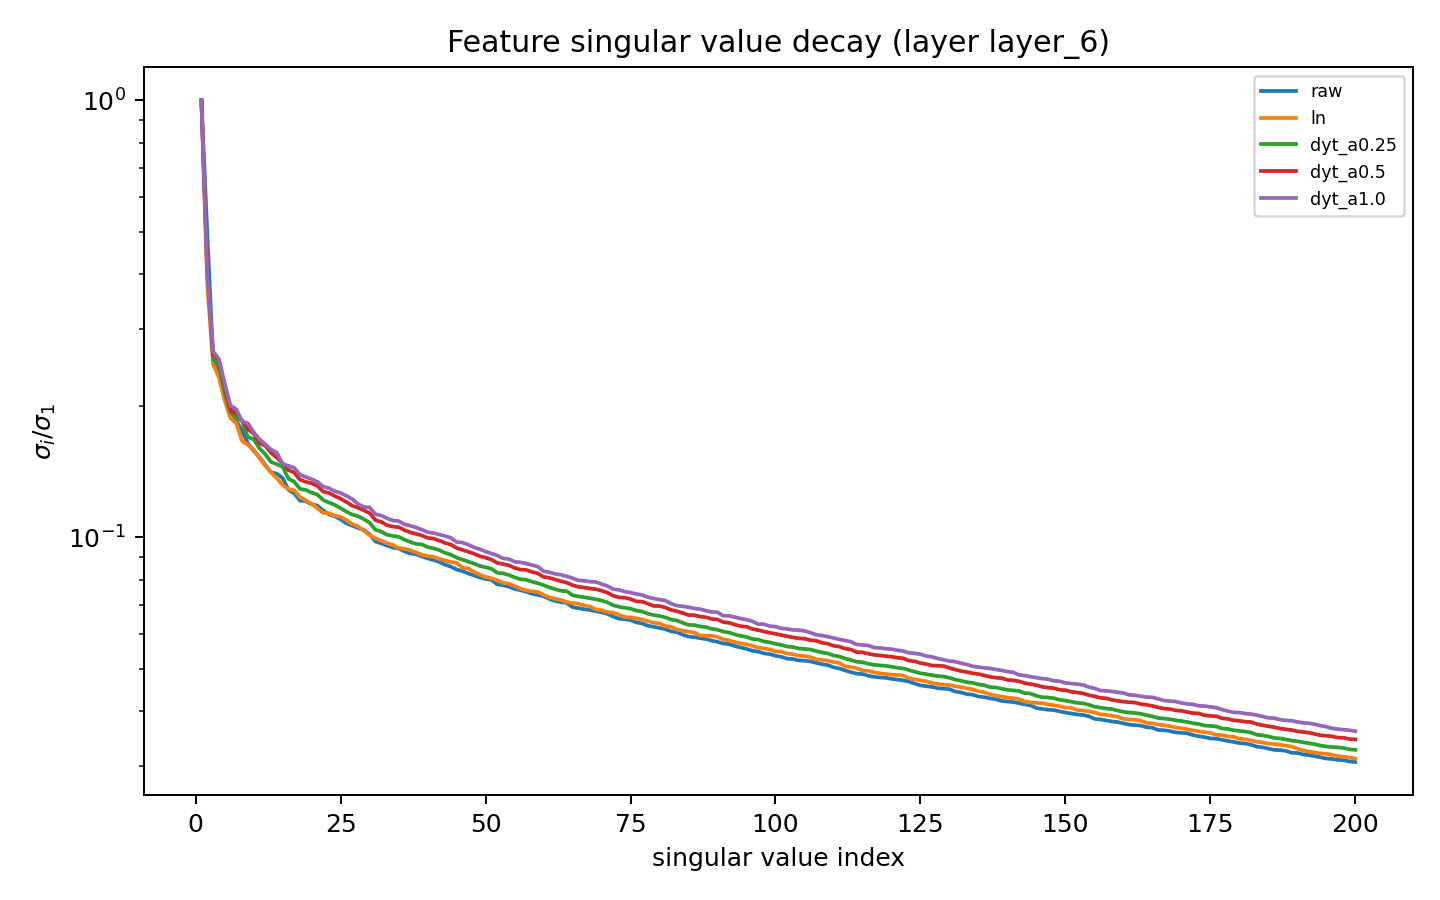
\includegraphics[width=0.7\linewidth]{results/fig_spectrum_X_final.png}
\caption{Normalized singular value decay $\sigma_i/\sigma_1$ for the final-layer feature matrix $X_{\textsf{layer\_6},T}$ across the five transforms.}
\label{fig:spectrum-X}
\end{figure}

Table~\ref{tab:layer6-summary} collects the headline diagnostics at \textsf{layer\_6} and is referenced throughout the remaining subsections.

\begin{table}[h]
\centering
\begin{tabular}{lccccc}
\toprule
Diagnostic & raw & LN & DyT $\alpha{=}0.25$ & DyT $\alpha{=}0.5$ & DyT $\alpha{=}1.0$ \\
\midrule
$\operatorname{mean}(\operatorname{diag}(G))$ & $143.6$ & $\mathbf{768.0}$ & $7.9$ & $28.3$ & $91.4$ \\
$\operatorname{std}(\operatorname{diag}(G))$  & $41.4$  & $\mathbf{0.011}$ & $2.0$ & $7.1$ & $20.6$ \\
$\kappaeff(X)$    & $417$  & $547$    & $391$ & $363$ & $\mathbf{319}$ \\
$\srank(X)$       & $2.50$ & $2.40$   & $2.56$ & $2.67$ & $\mathbf{2.76}$ \\
$\operatorname{err}_{32}(X)$ & $\mathbf{0.493}$ & $0.512$ & $0.519$ & $0.534$ & $0.547$ \\
\bottomrule
\end{tabular}
\caption{Headline diagnostics at \textsf{layer\_6} for the five transforms. Bold denotes the winner of each row.}
\label{tab:layer6-summary}
\end{table}

\subsection{Gram Diagonal: Row-Norm Geometry Diverges}
\label{sec:results-gram}

The Gram diagonal sharply confirms both predictions of Section~\ref{sec:maps}. For LN, Equation~\eqref{eq:ln-gram-diagonal} predicts $G_{ii}=d=768$ exactly; across all seven hidden states the measured $\operatorname{mean}(\operatorname{diag}(G_{\ell,\LN}))$ matches $d$ up to the $\varepsilon$ regularization in \eqref{eq:experiment-ln} and floating-point error, with $\operatorname{std}(\operatorname{diag}(G))$ negligible relative to the mean. The raw row norms vary substantially (Figure~\ref{fig:gram-bars}), so this uniform diagonal is imposed by LN rather than inherited from the input. For DyT, Equation~\eqref{eq:dyt-gram-diagonal} predicts $0\le G_{ii}\le d$, and Figure~\ref{fig:gram-bars} shows this realized nontrivially: both the mean and std of $\operatorname{diag}(G)$ grow with $\alpha$, so the diagonal is not fixed but tunable.

\begin{figure}[h]
\centering
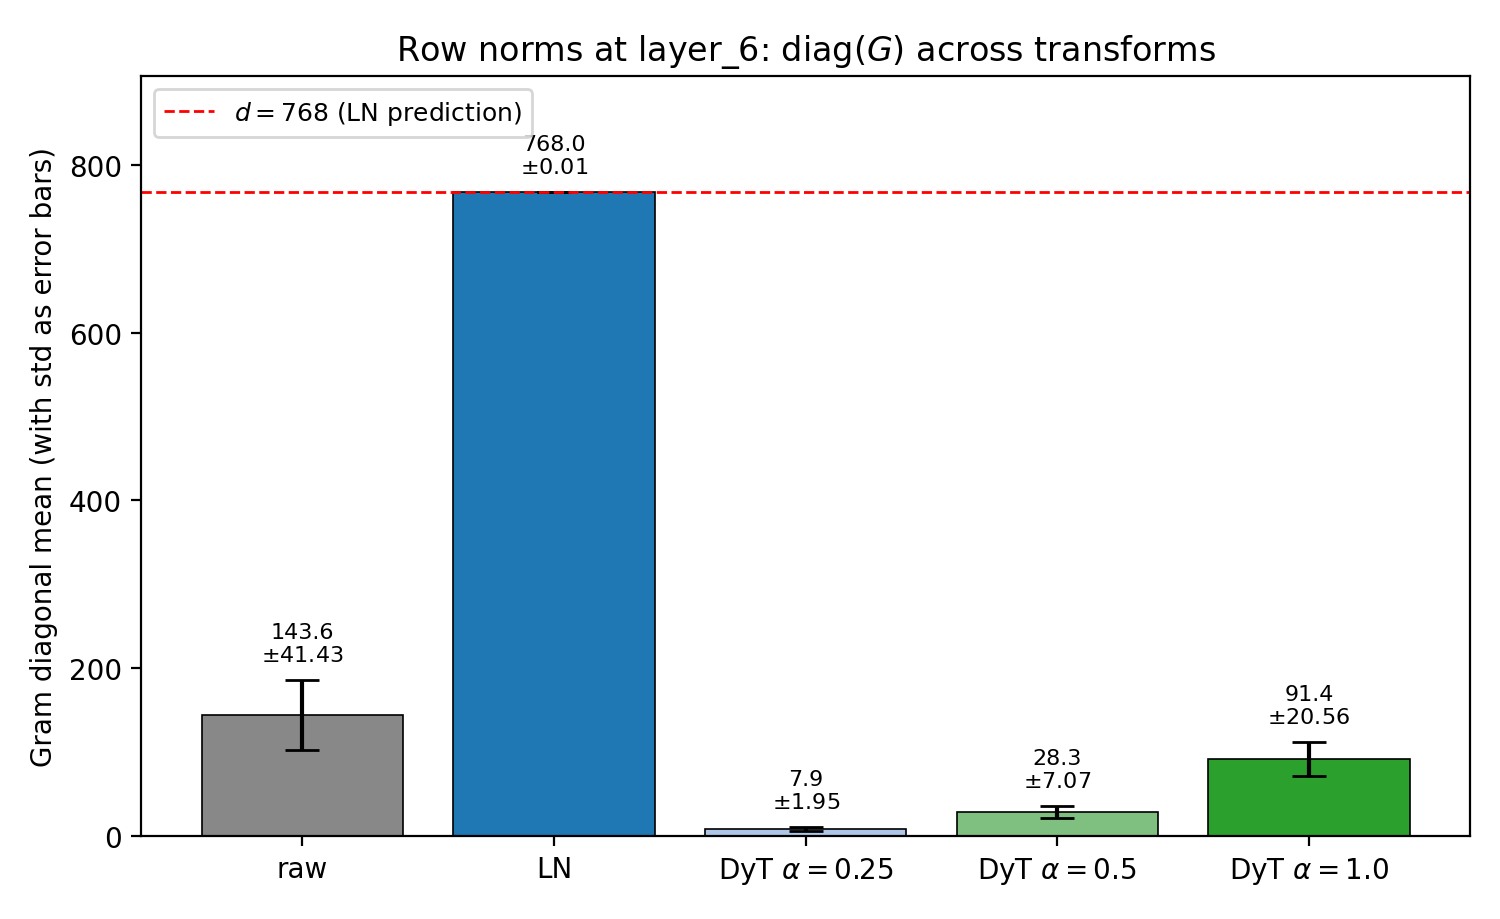
\includegraphics[width=0.7\linewidth]{results/fig_gram_diag_final_bars.png}
\caption{Gram diagonal at \textsf{layer\_6}: bar height is $\operatorname{mean}(\operatorname{diag}(G))$, error bars are one $\operatorname{std}$.}
\label{fig:gram-bars}
\end{figure}

\subsection{Spectral Conditioning: Normalization Does Not Uniformly Help}
\label{sec:results-conditioning}

Raw hidden states are poorly conditioned at most layers, and both transforms generally improve on this, but neither does so uniformly (Figure~\ref{fig:kappa-X}). At the output representation \textsf{layer\_6}, LN is actually worse conditioned than raw, while DyT improves on raw further; LN's clearest advantage is at \textsf{layer\_5}. The layer-by-layer ordering is irregular, so neither map confers a stable conditioning advantage on this sample. Section~\ref{sec:maps} did not claim LN was better conditioned, only that it removes shift and radial directions, and the data is consistent with that: those exact invariances can coincide with worse conditioning, sometimes even worse than no normalization at all. (The same ordering holds for $G$ at squared magnitudes, since $\kappa(G)=\kappa(X)^2$ on the nonzero spectral subspace.)

\begin{figure}[h]
\centering
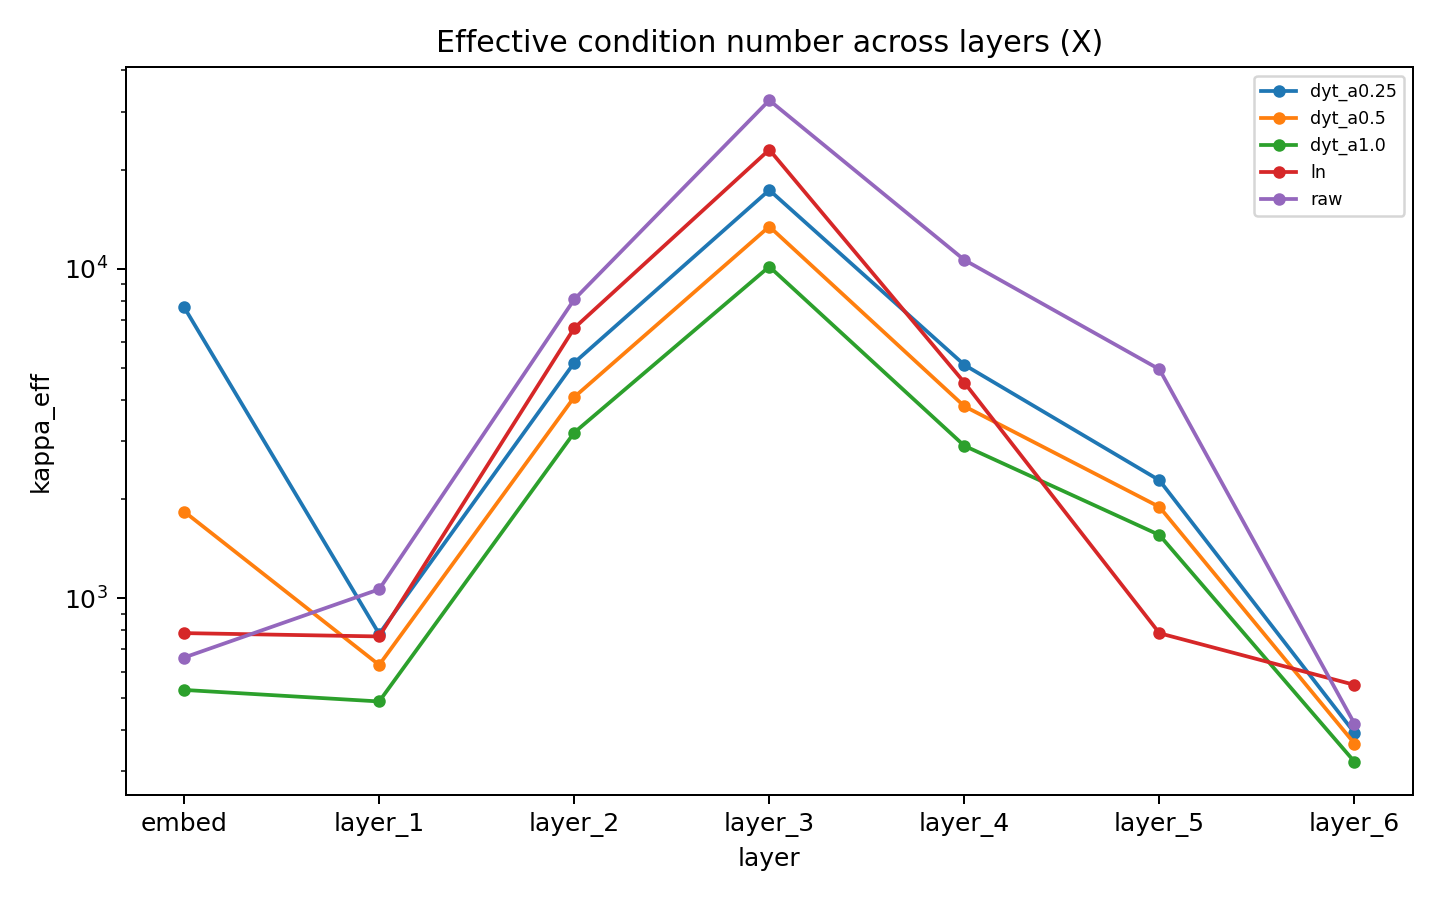
\includegraphics[width=0.75\linewidth]{results/fig_kappa_eff_X.png}
\caption{Effective condition number $\kappaeff(X_{\ell,T})$ across hidden states for the five transforms.}
\label{fig:kappa-X}
\end{figure}

\subsection{Spectral Compressibility: Stable Rank and Low-Rank Error}
\label{sec:results-rank}

Stable rank $\srank(X)$ is higher under DyT than under LN at every layer, and exceeds twice the LN value in earlier layers. Higher $\srank$ means spectral mass is spread across more directions rather than concentrated in $\sigma_1$. This is consistent with Section~\ref{sec:maps}: LN puts every row on the sphere of radius $\sqrt d$ in the mean-zero subspace, which aligns rows and inflates $\sigma_1$, whereas DyT only saturates coordinates. The rank-$32$ approximation error $\operatorname{err}_{32}(X)$ \eqref{eq:low-rank-error} differs by less than $0.06$ across the five transforms (Table~\ref{tab:layer6-summary}); LN and DyT do not change how well $X$ is approximated by a rank-$32$ matrix.

\subsection{Attention Scores and Perturbation Response}
\label{sec:results-attention}

Attention scores do not separate LN from DyT in the way the Gram diagonal does. At a $1\%$ relative perturbation of $Q$ and $K$, the mean response $\|\Delta S\|_F/\|S\|_F$ stays in the range $0.005$--$0.009$ across all transforms and all transformer layers; the \textsf{layer\_6} averages are $0.0059$ (raw), $0.0049$ (LN), $0.0068$ (DyT $\alpha=0.25$), $0.0079$ (DyT $\alpha=0.5$), and $0.0087$ (DyT $\alpha=1.0$). LN gives the smallest response and DyT responses grow with $\alpha$, but the spread between transforms is small relative to the $2\%$ input perturbation $\|\Delta Q\|_F/\|Q\|_F+\|\Delta K\|_F/\|K\|_F$, and all five values lie in the linear regime of the bound \eqref{eq:attention-relative-perturbation}. Stable rank of the per-head score matrix is also close: $\srank(S)$ for DyT $\alpha=1.0$ exceeds LN by $0.5$ at \textsf{layer\_6} and by at most $0.9$ in middle layers. So the row-level distinction at the input does not propagate to large structural differences in $S$ on this sample.

\section{Conclusion}

This paper recasts the LN-versus-DyT debate as a question about matrix-level numerical structure rather than downstream task accuracy. Section~\ref{sec:maps} separates the two maps cleanly at the row level: LN is a projection-rescaling that fixes row norms, removes the all-ones direction, and forces $G_{ii}=d$, while DyT is a coordinatewise saturation that only bounds rows. Section~\ref{sec:perturbation} provides a first-order bound on $\|\Delta S\|_2/\|S\|_2$ in terms of $\|\Delta Q\|_2,\|\Delta K\|_2$, used as the analytic tool for the attention experiments in Section~\ref{sec:results-attention}. Applied to DistilBERT, these tools deliver a split: the Gram diagonal $G_{ii}$ is the diagnostic where LN and DyT visibly diverge; stable rank $\srank(X)$ separates the maps systematically (DyT $>$ LN at every layer); the effective condition number $\kappaeff(X)$ separates them with no consistent layer ordering; and rank-$32$ approximation error $\operatorname{err}_{32}(X)$ together with the relative attention perturbation $\|\Delta S\|_F/\|S\|_F$ are close across all transforms.

These results give the practitioner a sharper picture of what is at stake when swapping LN for DyT. Task-level equivalence is consistent with row-level disagreement: anything that depends on row isometry (similarity caches, retrieval indices, geometry-aware probes) is sensitive to the choice of map, while anything that depends on the singular-value envelope of $X$ or on $\|\Delta S\|_F/\|S\|_F$ is largely indifferent to it. The same diagnostics extend directly to other normalization variants (RMSNorm, scaled-tanh, learned-$\alpha$ DyT) and to attention-score behavior under softmax, opening a route to ranking normalization choices by structural fingerprint rather than by benchmark numbers alone.

\bibliographystyle{plainnat}

\begin{thebibliography}{9}

\bibitem{ba2016layer}
Jimmy Lei Ba, Jamie Ryan Kiros, and Geoffrey E. Hinton.
\newblock Layer Normalization.
\newblock \emph{arXiv preprint arXiv:1607.06450}, 2016.

\bibitem{carroll1865alice}
Lewis Carroll.
\newblock Alice's Adventures in Wonderland.
\newblock Project Gutenberg eBook 11, public-domain text, 1865.
\newblock \url{https://www.gutenberg.org/ebooks/11}.

\bibitem{eckart1936approximation}
Carl Eckart and Gale Young.
\newblock The approximation of one matrix by another of lower rank.
\newblock \emph{Psychometrika}, 1:211--218, 1936.

\bibitem{shleifer2021normformer}
Sam Shleifer, Jason Weston, and Myle Ott.
\newblock NormFormer: Improved Transformer Pretraining with Extra Normalization.
\newblock \emph{arXiv preprint arXiv:2110.09456}, 2021.

\bibitem{vaswani2017attention}
Ashish Vaswani, Noam Shazeer, Niki Parmar, Jakob Uszkoreit,
Llion Jones, Aidan N. Gomez, Lukasz Kaiser, and Illia Polosukhin.
\newblock Attention Is All You Need.
\newblock In \emph{Advances in Neural Information Processing Systems}, 2017.

\bibitem{wang2022deepnet}
Hongyu Wang, Shuming Ma, Li Dong, Shaohan Huang, Dongdong Zhang, and Furu Wei.
\newblock DeepNet: Scaling Transformers to 1,000 Layers.
\newblock \emph{arXiv preprint arXiv:2203.00555}, 2022.

\bibitem{xiong2020layernorm}
Ruibin Xiong, Yunchang Yang, Di He, Kai Zheng, Shuxin Zheng, Chen Xing,
Huishuai Zhang, Yanyan Lan, Liwei Wang, and Tie-Yan Liu.
\newblock On Layer Normalization in the Transformer Architecture.
\newblock In \emph{International Conference on Machine Learning}, 2020.

\bibitem{zhang2019rmsnorm}
Biao Zhang and Rico Sennrich.
\newblock Root Mean Square Layer Normalization.
\newblock In \emph{Advances in Neural Information Processing Systems}, 2019.

\bibitem{zhu2025transformers}
Jiachen Zhu, Xinlei Chen, Kaiming He, Yann LeCun, and Zhuang Liu.
\newblock Transformers without Normalization.
\newblock In \emph{Proceedings of the IEEE/CVF Conference on Computer Vision and Pattern Recognition},
pages 14901--14911, 2025.

\end{thebibliography}

\end{document}
